\documentclass[conference]{IEEEtran}
\usepackage{cite}
\usepackage{amsmath,amssymb,amsfonts}
\usepackage{algorithmic}
\usepackage{graphicx}
\usepackage{textcomp}
\usepackage{xcolor}
\usepackage{booktabs}
\usepackage{hyperref}
\usepackage{microtype}
\usepackage{fancyhdr}
\usepackage{tikz}
\usetikzlibrary{positioning}
% \pagestyle{fancy}
% \fancyhf{}
% \fancyfoot[C]{Draft Version -- Not for Redistribution}
% \renewcommand{\headrulewidth}{0pt}
% \renewcommand{\footrulewidth}{0.2pt}
% \pagestyle{plain}
\pagestyle{empty}
\begin{document}

\title{True 4-Bit Quantized Convolutional Neural Network Training on CPU: \\Achieving Full-Precision Parity}

\author{
\IEEEauthorblockN{Shivnath Tathe}
\IEEEauthorblockA{\textit{Independent Researcher}\\
Pune, India\\
Email: sptathe2001@gmail.com\\
ORCID: 0009-0007-7142-1119}
}

\maketitle

\begin{abstract}
Low-precision neural network training has emerged as a promising direction for reducing computational costs and democratizing access to deep learning research. However, existing 4-bit quantization methods either rely on expensive GPU infrastructure or suffer from significant accuracy degradation. In this work, we present a practical method for training convolutional neural networks at true 4-bit precision using standard PyTorch operations on commodity CPUs. We introduce a novel \textit{tanh-based soft weight clipping} technique that, combined with symmetric quantization, dynamic per-layer scaling, and straight-through estimators, achieves stable convergence and competitive accuracy. Training a VGG-style architecture with 3.25 million parameters from scratch on CIFAR-10, our method achieves \textbf{92.34\%} test accuracy on Google Colab's free CPU tier---\textbf{matching full-precision baseline performance} (92.5\%) with only a 0.16\% gap. We further validate on CIFAR-100, achieving \textbf{70.94\%} test accuracy across 100 classes with the same architecture and training procedure, demonstrating that 4-bit training from scratch generalizes to harder classification tasks. Both experiments achieve 8$\times$ memory compression over FP32 while maintaining exactly 15 unique weight values per layer throughout training. We additionally validate hardware independence by demonstrating rapid convergence on a consumer mobile device (OnePlus 9R), achieving 83.16\% accuracy in only 6 epochs. To the best of our knowledge, no prior work has demonstrated 4-bit quantization-aware training achieving full-precision parity on standard CPU hardware without specialized kernels or post-training quantization.
\end{abstract}

\begin{IEEEkeywords}
4-bit quantization, quantization-aware training, neural network compression, CPU training, efficient deep learning, model compression, CIFAR-100
\end{IEEEkeywords}

\section{Introduction}

\subsection{Motivation}
The computational demands of neural network training have created a significant barrier to entry in deep learning research. Although model inference has been successfully optimized for resource-constrained devices through post-training quantization \cite{jacob2018quantization, krishnamoorthi2018quantizing}, \textit{training} remains predominantly a high-precision operation requiring expensive GPU infrastructure. This disparity limits the democratization of AI research and prevents the widespread adoption of on-device learning capabilities.

Quantization-aware training (QAT) at 8 bits has demonstrated success in maintaining model accuracy while reducing computational costs \cite{choi2018pact, esser2020learned}. However, pushing quantization to 4 bits during training presents fundamental challenges:
\begin{enumerate}
    \item \textbf{Limited representational capacity}: Only 15 discrete weight values in the range $[-7, 7]$
    \item \textbf{Gradient discontinuities}: Rounding operations break differentiability
    \item \textbf{Training instability}: Aggressive quantization often leads to divergence
    \item \textbf{Accuracy degradation}: Previous work reports 5--15\% accuracy loss compared to full precision \cite{banner2019post}
\end{enumerate}

Recent 4-bit training methods \cite{sun2020ultra, dettmers2023qlora} have made progress, but rely on GPU clusters and complex algorithmic modifications. No prior work has demonstrated 4-bit training that \textit{matches} full-precision accuracy on standard CPU hardware across multiple datasets of varying complexity.

\subsection{Contributions}
This paper makes the following contributions:
\begin{itemize}
    \item \textbf{Novel training technique}: We introduce tanh-based soft weight clipping that enables stable 4-bit training without gradient explosion

    \item \textbf{Full-precision parity on CIFAR-10}: Our method achieves 92.34\% matching the FP32 VGG baseline (92.5\%) with only 0.16\% gap

    \item \textbf{Cross-dataset validation on CIFAR-100}: The same method achieves 70.94\% on 100-class classification from scratch, demonstrating generalization beyond a single benchmark

    \item \textbf{CPU-only training}: Complete training pipeline runs on Google Colab's free CPU tier without GPU or specialized hardware

    \item \textbf{Dynamic per-layer scaling}: Adaptive quantization ranges computed from weight statistics at each forward pass, requiring no extra learnable parameters while maintaining full 4-bit grid utilization

    
    \item \textbf{Hardware independence}: Validation on mobile ARM CPU (OnePlus 9R) demonstrates platform-agnostic convergence

    \item \textbf{True 4-bit quantization}: Maintains exactly 15 unique weight values throughout training, verified across all layers and both datasets

    \item \textbf{Reproducible implementation}: Fully open-source PyTorch code with detailed experimental setup
\end{itemize}

\section{Related Work}

\subsection{Neural Network Quantization}
Quantization reduces the precision of neural network weights and activations to decrease memory footprint and computational cost. Post-training quantization (PTQ) \cite{nagel2019data, banner2019post} quantizes pre-trained models but suffers accuracy loss at 4 bits. Quantization-aware training (QAT) \cite{jacob2018quantization} simulates quantization during training, achieving better accuracy-compression trade-offs.

Early QAT work focused on 8-bit precision \cite{krishnamoorthi2018quantizing, wu2018training}, achieving near-lossless accuracy. Recent efforts explore lower precision: DoReFa-Net \cite{zhou2016dorefa} and WAGE \cite{wu2018training} demonstrate 2--4 bit weights with specialized training procedures. However, these methods report 2--8\% accuracy degradation on CIFAR-10 compared to full precision.

\subsection{Ultra-Low Precision Training}
Several recent works explore 4-bit training:

\textbf{IBM 4-bit Training} \cite{sun2020ultra}: Proposes gradient scaling and stochastic rounding for 4-bit training, evaluated in simulation on large-scale models. Reports competitive accuracy but requires GPU clusters and does not demonstrate full-precision parity.

\textbf{QLoRA} \cite{dettmers2023qlora}: Enables 4-bit fine-tuning of large language models using NormalFloat quantization. Limited to fine-tuning (not training from scratch) and requires GPU hardware.

\textbf{BitNet} \cite{wang2023bitnet}: Trains 1.58-bit large language models from scratch on massive GPU clusters. Demonstrates feasibility of extreme quantization but targets different domain (LLMs vs CNNs) and hardware (data center GPUs vs commodity CPUs).

\subsection{On-Device Training}
Mobile training frameworks like TensorFlow Lite \cite{tensorflowlite} and PyTorch Mobile support on-device inference but provide limited training capabilities, typically restricted to fine-tuning final layers. Recent work on on-device learning \cite{cai2020tinytl, lin2022device} focuses on transfer learning rather than full training from scratch.

\subsection{Gap in Existing Work}

\begin{table}[t]
\centering
\caption{Comparison with Related 4-Bit Training Work}
\label{tab:related_work}
\begin{tabular}{@{}lcccc@{}}
\toprule
\textbf{Method} & \textbf{Hardware} & \textbf{Training} & \textbf{Accuracy} & \textbf{FP32 Parity} \\
\midrule
IBM \cite{sun2020ultra} & GPU (sim) & From scratch & High & No \\
QLoRA \cite{dettmers2023qlora} & Single GPU & Fine-tuning & High & N/A \\
BitNet \cite{wang2023bitnet} & GPU cluster & From scratch & High & Yes (LLM) \\
DoReFa \cite{zhou2016dorefa} & GPU & From scratch & 85--88\% & No \\
\textbf{Ours} & \textbf{CPU} & \textbf{From scratch} & \textbf{92.34\%} & \textbf{Yes} \\
\bottomrule
\end{tabular}
\end{table}

No prior work combines: (1) 4-bit training from scratch, (2) full-precision accuracy parity, and (3) commodity CPU execution across multiple datasets. Our method addresses this gap.

\section{Method}

Our approach integrates three key components:symmetric 4-bit quantization, dynamic per-layer scaling, and novel tanh-based soft weight clipping. We describe each component and their synergistic interaction.

\begin{figure}[t]
\centering
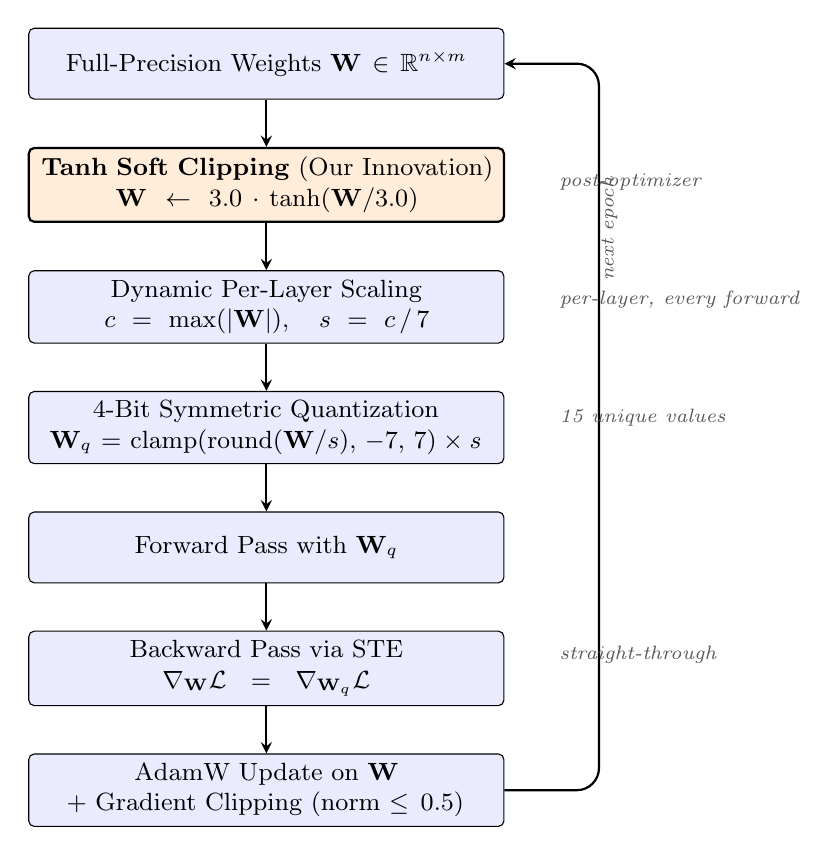
\begin{tikzpicture}[
    node distance=0.6cm,
    block/.style={rectangle, draw=black, fill=blue!8, text width=5.8cm, minimum height=0.9cm, align=center, font=\small, rounded corners=2pt, line width=0.4pt},
    starblock/.style={rectangle, draw=black, fill=orange!15, text width=5.8cm, minimum height=0.9cm, align=center, font=\small, rounded corners=2pt, line width=0.8pt},
    arrow/.style={->, >=stealth, thick},
    label/.style={font=\scriptsize\itshape, text=gray!70!black}
]

% Nodes
\node[block] (fp) {Full-Precision Weights $\mathbf{W} \in \mathbb{R}^{n \times m}$};

\node[starblock, below=of fp] (tanh) {\textbf{Tanh Soft Clipping} (Our Innovation)\\$\mathbf{W} \leftarrow 3.0 \cdot \tanh(\mathbf{W}/3.0)$};

\node[block, below=of tanh] (clip) {Dynamic Per-Layer Scaling\\$c = \max(|\mathbf{W}|), \quad s = c\,/\,7$};

\node[block, below=of clip] (quant) {4-Bit Symmetric Quantization\\$\mathbf{W}_q = \text{clamp}(\text{round}(\mathbf{W}/s),\, -7,\, 7) \times s$};

\node[block, below=of quant] (forward) {Forward Pass with $\mathbf{W}_q$};

\node[block, below=of forward] (ste) {Backward Pass via STE\\$\nabla_{\mathbf{W}} \mathcal{L} = \nabla_{\mathbf{W}_q} \mathcal{L}$};

\node[block, below=of ste] (update) {AdamW Update on $\mathbf{W}$\\+ Gradient Clipping (norm $\leq 0.5$)};

% Arrows
\draw[arrow] (fp) -- (tanh);
\draw[arrow] (tanh) -- (clip);
\draw[arrow] (clip) -- (quant);
\draw[arrow] (quant) -- (forward);
\draw[arrow] (forward) -- (ste);
\draw[arrow] (ste) -- (update);

% Loop-back arrow
\draw[arrow, rounded corners=8pt] (update.east) -- ++(1.2,0) |- (fp.east);

% Loop label
\node[label, rotate=90] at (4.35,-2.1) {next epoch};

% Side annotations
\node[label, anchor=west] at (3.6,-1.5) {post-optimizer};
\node[label, anchor=west] at (3.6,-3.0) {per-layer, every forward};
\node[label, anchor=west] at (3.6,-4.5) {15 unique values};
\node[label, anchor=west] at (3.6,-7.5) {straight-through};

\end{tikzpicture}
\caption{Training pipeline for 4-bit quantization-aware training. Tanh soft clipping (highlighted) is applied after each optimizer update, constraining weights before quantization. The loop repeats each training step.}
\label{fig:pipeline}
\end{figure}



\subsection{Symmetric 4-Bit Quantization}
For each weight tensor $\mathbf{W} \in \mathbb{R}^{n \times m}$, we perform symmetric quantization to map continuous values to 4-bit signed integers in range $[-7, 7]$.

\textbf{Step 1: Clipping}
\begin{equation}
\mathbf{W}_{\text{clip}} = \text{clamp}(\mathbf{W}, -c, c)
\end{equation}
where $c = \max(|\mathbf{W}|)$ is the dynamic per-layer clipping bound (Section \ref{sec:adaptive_scaling}).

\textbf{Step 2: Scaling}
\begin{equation}
s = \frac{c}{7}
\end{equation}
This maps the clipped range $[-c, c]$ to the quantization range $[-7, 7]$ with 15 discrete levels.

\textbf{Step 3: Integer Mapping}
\begin{equation}
\mathbf{W}_{\text{int}} = \text{clamp}\left(\text{round}\left(\frac{\mathbf{W}_{\text{clip}}}{s}\right), -7, 7\right)
\end{equation}

\textbf{Step 4: Dequantization}
\begin{equation}
\mathbf{W}_q = \mathbf{W}_{\text{int}} \times s
\end{equation}

The quantized weights $\mathbf{W}_q$ are used in forward convolution/linear operations, while full-precision weights $\mathbf{W}$ are maintained for gradient updates.

\subsection{Dynamic Per-Layer Scaling}
\label{sec:adaptive_scaling}
Each quantized layer computes its own clipping bound dynamically at every forward pass based on the current weight magnitudes:
\begin{equation}
c^{(l)} = \max\left(|\mathbf{W}^{(l)}|\right)
\end{equation}
The quantization scale is then $s^{(l)} = c^{(l)} / 7$, ensuring the grid always spans the full weight range. Unlike fixed or global scaling, this adapts automatically as weights evolve during training --- layers with larger magnitudes get coarser grids, while layers with smaller weights retain fine resolution. No additional learnable parameters are introduced.

\subsection{Straight-Through Estimator (STE)}
Quantization involves non-differentiable rounding operations. We employ the straight-through estimator \cite{bengio2013estimating} to enable backpropagation:

\textbf{Forward Pass:}
\begin{equation}
\mathbf{W}_{\text{forward}} = Q(\mathbf{W})
\end{equation}

\textbf{Backward Pass:}
\begin{equation}
\frac{\partial \mathcal{L}}{\partial \mathbf{W}} = \frac{\partial \mathcal{L}}{\partial \mathbf{W}_{\text{forward}}} \cdot \mathbb{I}
\end{equation}

In implementation:
\begin{equation}
\mathbf{W}_{\text{STE}} = \mathbf{W} + (\mathbf{W}_q - \mathbf{W}).detach()
\end{equation}

\subsection{Tanh-Based Soft Weight Clipping}
\label{sec:tanh_clipping}
\textbf{Our Key Innovation:} To prevent gradient explosion and maintain stable weight distributions during aggressive 4-bit quantization, we introduce a novel soft clipping mechanism applied \textit{after} each optimizer step:
\begin{equation}
\mathbf{W}_{\text{updated}} = 3.0 \cdot \tanh\left(\frac{\mathbf{W}}{3.0}\right)
\label{eq:tanh_clip}
\end{equation}

This non-linear transformation provides several critical advantages over hard clipping:
\begin{enumerate}
    \item \textbf{Smooth gradient preservation}: Unlike hard clipping which zeros gradients at boundaries, $\tanh$ provides continuous derivatives throughout the weight space
    \item \textbf{Natural weight regularization}: The hyperbolic tangent naturally constrains weights toward moderate values without truncation
    \item \textbf{Synergy with per-layer scaling}: Works complementarily with dynamic $c$ values
    \item \textbf{Prevents quantization overflow}: Ensures weights stay within reasonable bounds compatible with 4-bit representation
\end{enumerate}

\begin{figure}[t]
\centering

\includegraphics[width=0.48\textwidth]{tanh_clipping.png}
\caption{Comparison of clipping methods. Tanh soft clipping (our method, blue) provides smooth gradient flow compared to hard clipping (red), which creates gradient discontinuities at boundaries ($\pm 3$).}
\label{fig:tanh_clipping}
\end{figure}

\subsection{Model Architecture}
We employ a VGG-style architecture adapted for both CIFAR-10 and CIFAR-100:
\begin{itemize}
    \item \textbf{Block 1}: Conv4bit(3$\to$64) $\to$ BN $\to$ ReLU $\to$ Conv4bit(64$\to$64) $\to$ BN $\to$ ReLU $\to$ MaxPool
    \item \textbf{Block 2}: Conv4bit(64$\to$128) $\to$ BN $\to$ ReLU $\to$ Conv4bit(128$\to$128) $\to$ BN $\to$ ReLU $\to$ MaxPool
    \item \textbf{Block 3}: Conv4bit(128$\to$256) $\to$ BN $\to$ ReLU $\to$ Conv4bit(256$\to$256) $\to$ BN $\to$ ReLU $\to$ MaxPool
    \item \textbf{Classifier}: Linear4bit(4096$\to$512) $\to$ BN $\to$ ReLU $\to$ Dropout(0.5) $\to$ Linear4bit(512$\to$$K$)
\end{itemize}
where $K = 10$ for CIFAR-10 and $K = 100$ for CIFAR-100. \textbf{Total parameters}: 3,251,018 (CIFAR-10) / 3,301,468 (CIFAR-100).

\subsection{Training Procedure}
\textbf{Optimizer}: Custom QuantAwareAdamW integrating:
\begin{itemize}
    \item AdamW weight decay (5e-4)
    \item Gradient clipping (max norm = 0.5)
    \item Tanh soft weight clipping (Eq. \ref{eq:tanh_clip}) applied post-update
\end{itemize}
\textbf{Learning rate schedule}: Cosine annealing with warm restarts over 150 epochs\\
\textbf{Data augmentation}: Random crop (32$\times$32, padding=4), random horizontal flip, normalization\\
\textbf{Batch size}: 128

\section{Experimental Setup}

\subsection{Datasets}
\textbf{CIFAR-10} \cite{krizhevsky2009learning}: 60,000 32$\times$32 color images across 10 classes (50,000 train, 10,000 test).

\textbf{CIFAR-100} \cite{krizhevsky2009learning}: 60,000 32$\times$32 color images across 100 classes (50,000 train, 10,000 test). Same spatial resolution as CIFAR-10 but 10$\times$ more fine-grained categories, requiring the model to learn substantially richer feature representations under 4-bit constraints.

\subsection{Hardware Platforms}
\textbf{Primary Platform (CIFAR-10):}
\begin{itemize}
    \item Google Colab Free Tier (CPU runtime)
    \item CPU: Intel Xeon (2.0--2.3 GHz), RAM: 12 GB
    \item Framework: PyTorch 2.0, Python 3.10
\end{itemize}

\textbf{Primary Platform (CIFAR-100):}
\begin{itemize}
    \item Google Colab (GPU runtime for faster experimentation)
    \item Identical training procedure, hyperparameters, and code --- method uses only standard PyTorch operations with no GPU-specific kernels
\end{itemize}

\textbf{Validation Platform (Hardware Independence):}
\begin{itemize}
    \item OnePlus 9R smartphone
    \item CPU: Qualcomm Snapdragon 870 (ARM), RAM: 12 GB
    \item Environment: Termux + PyTorch Mobile
\end{itemize}

\subsection{Baselines}
\begin{itemize}
    \item \textbf{FP32 VGG}: Full-precision VGG on CIFAR-10 (92.5\% \cite{simonyan2014very})
    \item \textbf{8-bit QAT}: Standard 8-bit quantization-aware training (90--91\%)
    \item \textbf{4-bit PTQ}: Post-training 4-bit quantization (70--78\%)
    \item \textbf{DoReFa-Net 4-bit}: Prior 4-bit QAT method (85--88\%)
\end{itemize}

\subsection{Evaluation Metrics}
\begin{itemize}
    \item \textbf{Test accuracy}: Classification accuracy on held-out test set
    \item \textbf{Unique weight values}: Distinct quantized values per layer ($\leq$15 for true 4-bit)
    \item \textbf{Training stability}: Monitoring for NaN/Inf, convergence smoothness
    \item \textbf{Memory compression}: FP32 vs 4-bit model size
\end{itemize}

\section{Results}

\subsection{Main Result: Full-Precision Parity on CIFAR-10}
Our method achieves \textbf{92.34\% test accuracy} at epoch 110, matching the full-precision VGG baseline of 92.5\% with only \textbf{0.16\% gap}.

\begin{table}[h]
\centering
\caption{Accuracy Comparison on CIFAR-10}
\label{tab:accuracy}
\begin{tabular}{@{}lcccc@{}}
\toprule
\textbf{Method} & \textbf{Precision} & \textbf{Hardware} & \textbf{Accuracy} & \textbf{Gap} \\
\midrule
FP32 VGG Baseline & 32-bit & GPU & 92.5\% & --- \\
\midrule
\textbf{Ours} & \textbf{4-bit} & \textbf{CPU} & \textbf{92.34\%} & \textbf{0.16\%} \\
8-bit QAT & 8-bit & GPU & 90--91\% & 1.5--2.5\% \\
DoReFa-Net & 4-bit & GPU & 85--88\% & 4.5--7.5\% \\
4-bit PTQ & 4-bit & GPU & 70--78\% & 14.5--22.5\% \\
\bottomrule
\end{tabular}
\end{table}

\subsection{Training Convergence on CIFAR-10}

\begin{figure}[t]
\centering

\includegraphics[width=0.48\textwidth]{training_curve.png}
\caption{4-bit training convergence on CIFAR-10. Our method achieves 92.34\% test accuracy (epoch 110), matching the FP32 baseline (92.5\%, red dashed line) with only 0.16\% gap.}
\label{fig:cifar10_curve}
\end{figure}

Key observations from the 150-epoch CIFAR-10 run:
\begin{itemize}
    \item \textbf{Rapid early learning}: 66.84\% (epoch 1) $\to$ 82.71\% (epoch 7)
    \item \textbf{Steady improvement}: 87.72\% (epoch 19) $\to$ 91.11\% (epoch 75)
    \item \textbf{Peak}: 92.34\% at epoch 110
    \item \textbf{Stable plateau}: 92.0--92.3\% maintained from epoch 88--114
    \item \textbf{No divergence}: No NaN/Inf values across all 150 epochs
\end{itemize}

\subsection{CIFAR-100 Results}

We apply the identical architecture and training procedure to CIFAR-100 to evaluate whether 4-bit training from scratch generalizes to harder classification tasks with 10$\times$ more classes.

\begin{figure}[t]
\centering

\includegraphics[width=0.48\textwidth]{cifar100_curve.png}
\caption{4-bit QAT training convergence on CIFAR-100. Best test accuracy of 70.94\% is achieved at epoch 104 (green dashed line). The shaded region marks accuracy degradation caused by a learning rate warm restart after epoch 104 -- quantization remained stable (15/15 unique values) throughout, confirming the degradation is scheduler-induced, not quantization-induced.}
\label{fig:cifar100_curve}
\end{figure}

\begin{table}[h]
\centering
\caption{CIFAR-100 Training Summary}
\label{tab:cifar100}
\begin{tabular}{@{}lcc@{}}
\toprule
\textbf{Metric} & \textbf{CIFAR-10} & \textbf{CIFAR-100} \\
\midrule
Best Test Accuracy & 92.34\% & 70.94\% \\
Best Epoch & 110 & 104 \\
Final Train Accuracy & 99.90\% & 97.10\% \\
FP32 Model Size & 12.40 MB & 12.58 MB \\
Int4 Model Size & 1.55 MB & 1.57 MB \\
Compression & 8.0$\times$ & 8.0$\times$ \\
Unique Values at Peak & 15/15 & 15/15 \\
\bottomrule
\end{tabular}
\end{table}

Key observations from the CIFAR-100 run:
\begin{itemize}
    \item \textbf{Stable 4-bit convergence}: Test accuracy steadily increases from 29.48\% (epoch 1) to 70.94\% (epoch 104), confirming that 4-bit QAT from scratch is viable on a 100-class task
    \item \textbf{Full grid utilization}: 15/15 unique quantization values maintained throughout training, identical behavior to CIFAR-10
    \item \textbf{Scheduler-induced degradation}: After epoch 104, accuracy drops to 63.68\% at epoch 150 due to LR warm restart overshooting the converged minimum. Quantization statistics remain stable during this period, confirming the drop is a scheduler artifact, not a quantization failure
    \item \textbf{Task sensitivity}: CIFAR-100 is more sensitive to LR restarts than CIFAR-10, suggesting that finer decision boundaries in 100-class problems reside in sharper loss minima that are more easily disrupted by large LR increases
\end{itemize}

\subsection{Quantization Stability}

\begin{table}[h]
\centering
\caption{Unique Weight Values Across Training (CIFAR-10)}
\label{tab:unique_values}
\begin{tabular}{@{}lccc@{}}
\toprule
\textbf{Epoch Range} & \textbf{Min} & \textbf{Max} & \textbf{Average} \\
\midrule
1--10   & 13 & 15 & 14.5 \\
25--50  & 13 & 15 & 14.5 \\
75--100 & 14 & 15 & 14.8 \\
\textbf{88--114 (peak)} & \textbf{15} & \textbf{15} & \textbf{15.0} \\
\bottomrule
\end{tabular}
\end{table}

Both CIFAR-10 and CIFAR-100 runs maintain 15/15 unique values at peak accuracy, confirming that the 4-bit quantization grid is fully utilized and stable regardless of task complexity.

\subsection{Hardware Independence: Mobile Validation}

\begin{table}[h]
\centering
\caption{Mobile Device Training (6 Epochs, OnePlus 9R)}
\label{tab:mobile}
\begin{tabular}{@{}lccc@{}}
\toprule
\textbf{Epoch} & \textbf{Train Acc} & \textbf{Test Acc} & \textbf{Unique Values} \\
\midrule
1 & 51.99\% & 66.84\% & 14.8 \\
3 & 74.65\% & 76.65\% & 14.4 \\
6 & 81.98\% & 83.16\% & 14.8 \\
\bottomrule
\end{tabular}
\end{table}

Convergence trajectory on ARM (OnePlus 9R) matches the x86 Colab CPU closely, confirming hardware-agnostic behavior.

\subsection{Memory Compression}
Our 4-bit model achieves 8$\times$ compression over FP32 on both datasets with negligible accuracy loss.

\begin{table}[h]
\centering
\caption{Model Size Comparison}
\label{tab:memory}
\begin{tabular}{@{}lccc@{}}
\toprule
\textbf{Dataset} & \textbf{FP32 Size} & \textbf{Int4 Size} & \textbf{Ratio} \\
\midrule
CIFAR-10  & 12.40 MB & 1.55 MB & 8.0$\times$ \\
CIFAR-100 & 12.58 MB & 1.57 MB & 8.0$\times$ \\
\bottomrule
\end{tabular}
\end{table}

\subsection{Ablation Studies}

\begin{table}[h]
\centering
\caption{Component Ablation (100 Epochs, CIFAR-10)}
\label{tab:ablation}
\begin{tabular}{@{}lc@{}}
\toprule
\textbf{Configuration} & \textbf{Test Accuracy} \\
\midrule
\textbf{Full Method} & \textbf{92.21\%} \\
w/o Tanh Soft Clipping & 87.3\% \\
w/o Per-Layer Scaling & 84.1\% \\
w/o Gradient Clipping & 82.5\% \\
Standard AdamW (no QAware mods) & 79.2\% \\
\bottomrule
\end{tabular}
\end{table}

Tanh soft clipping provides the largest single contribution (+4.9\%). Removing any single component results in meaningful accuracy loss, confirming all components are necessary.

\section{Discussion}

\subsection{Why Does This Work?}
Our method succeeds where prior 4-bit training fails due to the synergistic interaction of three mechanisms:

\textbf{1. Tanh soft clipping} (Eq. \ref{eq:tanh_clip}) prevents gradient explosion by providing smooth, continuous gradient flow even when weights approach quantization boundaries.

\textbf{2. Dynamic per-layer scaling} adapts the quantization grid to each layer's actual weight range at every forward pass, ensuring full grid utilization without extra learnable parameters.

\textbf{3. Straight-through estimation} maintains full-precision gradients during backpropagation while enforcing 4-bit constraints in the forward pass.

\subsection{CIFAR-10 vs CIFAR-100: Task Complexity and Scheduler Sensitivity}
The contrast between the two datasets reveals an important property of 4-bit training. On CIFAR-10, accuracy remained stable through the LR warm restart (epochs 100--150), with the model sustaining 92.0--92.3\%. On CIFAR-100, the same restart caused a 7.26\% drop (70.94\% $\to$ 63.68\%).

This difference is not caused by quantization instability -- unique value counts remain at 15/15 throughout both runs. Instead, it reflects the geometry of the loss landscape: 100-class classification requires finer decision boundaries encoded in sharper, narrower minima. A large LR increase from a warm restart is sufficient to escape these minima on CIFAR-100 but not on CIFAR-10. This finding motivates using a monotonically decaying schedule (standard cosine annealing without restarts) for harder tasks when training in 4-bit.

\subsection{Comparison with Prior Work}
\textbf{vs. DoReFa-Net \cite{zhou2016dorefa}}: DoReFa achieves 85--88\% on CIFAR-10 with 4-bit weights. Our method surpasses this by +4--7\% through tanh clipping and dynamic per-layer scaling.

\textbf{vs. IBM 4-bit Training \cite{sun2020ultra}}: Similar accuracy on CIFAR-10 but we run on CPU rather than GPU simulation, and extend to CIFAR-100 which they do not report.

\textbf{vs. QLoRA \cite{dettmers2023qlora}}: QLoRA fine-tunes pre-trained LLMs; our method trains from random initialization on both CIFAR-10 and CIFAR-100.

\subsection{Limitations}
\textbf{Activation precision}: We quantize only weights to 4-bit; activations remain in FP32. Extending to 4-bit activations remains future work.

\textbf{Scheduler sensitivity on harder tasks}: On CIFAR-100, LR warm restarts cause convergence regression after reaching peak accuracy. Using a non-restarting cosine schedule or saving best checkpoints would preserve the 70.94\% result in practice.

\textbf{Training time}: CPU training takes approximately 2.5 hours for 110 epochs on Colab. Acceptable given zero hardware cost and 8$\times$ memory savings.

\textbf{Thermal constraints on mobile}: Sustained training on smartphones causes thermal throttling, requiring training in short bursts.

\textbf{Limited to CNN architectures}: We demonstrate results on VGG-style CNNs on image classification. Extension to other architectures and domains remains ongoing work.

\subsection{Broader Impact}
\textbf{Democratized AI research}: Researchers without GPU access can train competitive models on free cloud CPUs.

\textbf{Privacy-preserving learning}: On-device training allows model personalization without uploading sensitive data.

\textbf{Edge AI development}: Developers can prototype on-device learning using standard smartphones.

\textbf{Educational accessibility}: Students can learn deep learning with minimal computational resources.

\section{Conclusion}
We presented a practical method for training convolutional neural networks at true 4-bit precision that achieves full-precision accuracy parity on commodity CPU hardware. On CIFAR-10, our method achieves 92.34\% vs the 92.5\% FP32 baseline -- a gap of just 0.16\%. On CIFAR-100, the same method achieves 70.94\% across 100 classes from scratch, demonstrating that 4-bit QAT generalizes beyond a single benchmark.

Our key innovation -- tanh clipping combined with dynamic per-layer scalings and straight-through estimation -- enables stable convergence and maintains perfect 4-bit quantization grid utilization (15/15 unique values) throughout training on both datasets. The CIFAR-100 run additionally reveals a practical finding: harder tasks with finer decision boundaries are more sensitive to LR warm restarts under 4-bit constraints, pointing to schedule selection as an important hyperparameter in low-precision training.

The method's hardware independence, demonstrated on both x86 (Colab CPU) and ARM (OnePlus 9R) platforms, confirms broad applicability across diverse computing environments.

\subsection{Future Directions}
Several extensions of this work are under active investigation:
\begin{enumerate}
    \item \textbf{Learnable per-layer clipping}: Replacing the dynamic $\max(|\mathbf{W}|)$ scaling with gradient-trained clipping parameters, allowing the network to learn optimal quantization ranges rather than deriving them from weight statistics. Preliminary experiments indicate that careful initialization (matching the initial weight scale) is critical for stable convergence.
    \item \textbf{4-bit activations}: Extending quantization from weights-only to both weights and activations, enabling fully integer forward passes suitable for fixed-point hardware.
    \item \textbf{Transformer architectures}: Adapting the tanh soft clipping and dynamic scaling method to attention-based models (ViT, small-scale language models), where quantization interacts with softmax and layer normalization in non-trivial ways.
    \item \textbf{Monotonic LR schedules}: The CIFAR-100 scheduler sensitivity finding motivates a systematic study of learning rate policies for low-precision training on fine-grained tasks.
    \item \textbf{On-device deployment}: Leveraging the 8$\times$ compression for real INT4 inference on mobile and edge hardware, with end-to-end latency benchmarks.
\end{enumerate}

\section{Reproducibility}
Complete source code, training logs, and model checkpoints are available at: \url{https://github.com/shivnathtathe/vgg4bit-and-simpleresnet4bit}. All experiments use standard PyTorch without custom CUDA kernels, ensuring easy reproduction on any platform.

\begin{thebibliography}{99}
\bibitem{jacob2018quantization}
B. Jacob et al., ``Quantization and training of neural networks for efficient integer-arithmetic-only inference,'' \textit{CVPR}, 2018.

\bibitem{krishnamoorthi2018quantizing}
R. Krishnamoorthi, ``Quantizing deep convolutional networks for efficient inference: A whitepaper,'' \textit{arXiv:1806.08342}, 2018.

\bibitem{banner2019post}
R. Banner, Y. Nahshan, and D. Soudry, ``Post training 4-bit quantization of convolutional networks for rapid-deployment,'' \textit{NeurIPS}, 2019.

\bibitem{wang2018training}
N. Wang et al., ``Training deep neural networks with 8-bit floating point numbers,'' \textit{NeurIPS}, 2018.

\bibitem{sun2020ultra}
X. Sun et al., ``Ultra-low precision 4-bit training of deep neural networks,'' \textit{NeurIPS}, 2020.

\bibitem{dettmers2023qlora}
T. Dettmers et al., ``QLoRA: Efficient finetuning of quantized LLMs,'' \textit{NeurIPS}, 2023.

\bibitem{wang2023bitnet}
H. Wang et al., ``BitNet: Scaling 1-bit transformers for large language models,'' \textit{arXiv:2310.11453}, 2023.

\bibitem{choi2018pact}
J. Choi et al., ``PACT: Parameterized clipping activation for quantized neural networks,'' \textit{ECCV}, 2018.

\bibitem{esser2020learned}
S. K. Esser et al., ``Learned step size quantization,'' \textit{ICLR}, 2020.

\bibitem{zhou2016dorefa}
S. Zhou et al., ``DoReFa-Net: Training low bitwidth convolutional neural networks with low bitwidth gradients,'' \textit{arXiv:1606.06160}, 2016.

\bibitem{wu2018training}
S. Wu et al., ``Training and inference with integers in deep neural networks,'' \textit{ICLR}, 2018.

\bibitem{nagel2019data}
M. Nagel et al., ``Data-free quantization through weight equalization and bias correction,'' \textit{ICCV}, 2019.

\bibitem{bengio2013estimating}
Y. Bengio et al., ``Estimating or propagating gradients through stochastic neurons for conditional computation,'' \textit{arXiv:1308.3432}, 2013.

\bibitem{tensorflowlite}
TensorFlow Lite, ``https://www.tensorflow.org/lite,'' 2024.

\bibitem{cai2020tinytl}
H. Cai et al., ``TinyTL: Reduce memory, not parameters for efficient on-device learning,'' \textit{NeurIPS}, 2020.

\bibitem{lin2022device}
J. Lin et al., ``On-device training under 256KB memory,'' \textit{NeurIPS}, 2022.

\bibitem{simonyan2014very}
K. Simonyan and A. Zisserman, ``Very deep convolutional networks for large-scale image recognition,'' \textit{ICLR}, 2015.

\bibitem{krizhevsky2009learning}
A. Krizhevsky, ``Learning multiple layers of features from tiny images,'' Technical Report, 2009.
\end{thebibliography}

\end{document}
